\section{人体几何模型的应用}
\subsection{问题描述}
在上一部分中,我们已经从图片中得到人体的三维关节点的坐标,但是在实际应用中,简单的骨架表示不够具有表现力,因此最新的论文里的做法是使用一个预先生成好的参数化的人体几何模型,通过优化算法,或者直接通过网络估计,得到该模型的参数。在我们的问题中,希望通过输入一个人体的骨架的三维坐标,输出该参数化模型的参数。由于骨架坐标无法完全确定该模型的参数,因此我们需要引入一些额外的约束,来完成该求解过程。

\subsection{模型介绍}
SMPL模型是一个高效的线性人体模型,模型总共定义了\(N = 6890\)个顶点,作为人体的模板\(\bar{\bm{T}}\)。为了使该模型能够描述不同的人体姿态,该模型定义了人体的24个关节,每个关节具有三个旋转的自由度(包括整个身体的旋转),再加上身体的平移的三个自由度,该模型使用了\(3\times 24 + 3 = 75\)个位姿参数\(\theta\)来描述人体的姿态。为了能够描述不同人体的形状的差异,模型使用了形状参数\(\beta\)来对人体模板的点进行非刚性变形。也就是说,人体模板首先会根据形状参数和姿态参数进行变形:
\begin{equation}
    T(\beta, \theta) = \bar{\bm{T}} + B_S(\beta) + B_P(\theta)
\end{equation}
这里的\(B_S(\beta)\)是一个形状混合函数,他将形状参数\(\beta \in \mathbb{R}^{|\beta|}\)映射到人的模型的顶点所在的空间内,即\(B_S(\beta):\mathbb{R}^{|\beta|} \mapsto \mathbb{R}^{3N}\)。这里的\(B_P(\beta)\)是一个依赖于姿势的形状混合函数,他将姿势参数\(\theta \in \mathbb{R}^{|\theta|}\)同样映射到人的模型的顶点所在的空间内,即\(B_P(\beta):\mathbb{R}^{|\theta|} \mapsto \mathbb{R}^{3N}\),这一项考虑的是人体在进行不同的动作的时候,对身体的造成的形变。这两项形状混合函数都是直接将点的坐标加到人体的静止姿态下,也就是说先对人体的静止姿态进行变形,完成对形状的改变。在这之后,再对人体模型上的所有点进行混合蒙皮操作(blend skinning),将非关键点的位置进行旋转平移,得到经过姿势变换后的人体模型上的点的位置。

\textbf{混合蒙皮(Blend skinning):}这一步的目的是为了根据输入的姿态参数\(theta\)将人体的网格模型进行变形。人体的姿态参数的定义是,对于每个关节,使用轴角(axis-angle)来表示他的旋转。由于每一个旋转矩阵只有三个自由度,所以一般的表示方法都是使用参数化的表示。常用的参数化的方法是使用欧拉角,但是欧拉角会带来万向锁的问题,因为欧拉角表示并没有覆盖旋转矩阵空间内的所有区域。并且,欧拉角使用角度来进行表示,这样在进行优化的时候其值的范围是有周期性的,不连续,使得优化过程不自然,因此选择了使用轴角表示。

对于我们的骨架模型,有\(K=23\)个关节表示旋转,加上人整体的旋转,姿势参数即为\(\theta = [\omega_0^T, \omega_1^T, \ldots, \omega_K^T]\),其中的每一个\(\omega\)是一个三维的向量,\(\omega\)的模长\(||\omega||\)表示旋转的角度,\(\frac{\omega}{||\omega||}\)表示旋转的方向的单位向量。为了在计算的时候表示旋转,通常会需要先转换成旋转矩阵。旋转向量转化成旋转矩阵的方法是通过罗德里格斯公式(Rodrigues formula):
\begin{equation}
    \exp \left(  \omega  _ { j } \right) = \mathcal { I } + \widehat { \overline { \omega }} _ { j } \sin \left( \left\|  \omega  _ { j } \right\| \right) + \widehat { \overline { \omega } } _ { j } ^ { 2 } \cos \left( \left\| \omega_ { j } \right\| \right)
\end{equation}
其中\(\overline { \omega } = \frac{\omega}{||\omega||}\)表示旋转轴的单位向量,\(\widehat { \overline { \omega }}\)表示关于三维向量\(\overline{\omega}\)的反对称矩阵,即对于向量\(\mathbf{K} = [k_x, k_y, k_z]^T\),其计算公式为
\begin{equation}
\widehat{\mathbf { K }} = \left[ \begin{array} { c c c } { 0 } & { - k _ { z } } & { k _ { y } } \\ { k _ { z } } & { 0 } & { - k _ { x } } \\ { - k _ { y } } & { k _ { x } } & { 0 } \end{array} \right]
\end{equation}
\(\mathcal { I }\)表示\(3\times 3\)的单位矩阵。那么通过这一步计算,我们即将所有的\(K \times 3\)的旋转向量转换成了\(K\times 3 \times 3\)的旋转矩阵。由于在进行点的坐标计算的时候,一般都使用齐次坐标来表示点的位置,因此我们需要将旋转矩阵扩充为\(4\times 4\)的齐次变换矩阵。也即是说对于每个关节,都有一个局部的齐次变换矩阵,写为
\begin{equation}
\left[ \begin{array} { c | c } { \exp \left( \vec { \omega } _ { j } \right) } & { \mathbf { j } _ { j } } \\ \hline \overrightarrow { 0 } & { 1 } \end{array} \right]
\end{equation}
计算该关节相对于全局坐标系的齐次变换矩阵时,即需要根据骨架连接的顺序,依次将各个关节的局部变换矩阵相乘,即可得到该关节的全局变换矩阵,即
\begin{equation}
    G _ { k } ( \vec { \theta } , \mathbf { J } ) = \prod _ { j \in A ( k ) } \left[ \begin{array} { c | c } { \exp \left( \vec { \omega } _ { j } \right) } & { \mathbf { j } _ { j } } \\ \hline \overrightarrow { 0 } & { 1 } \end{array} \right]
\end{equation}
其中,\(A(k)\)表示对于关节\(k\),其所有父节点的按连接顺序排列的有序集合。\comment{插个图片,举个例子}。该式子表示,对于关节\(k\),其全局变换矩阵的计算为其父节点的全局变换矩阵的依次矩阵相乘。\(\mathbf{j}_j\)表示关节\(j\)的相对于其父节点的位移,其长度即为该段骨长。在计算时,考虑到在初始状态时模型的点的位置应该不发生改变,因此需要构造一个矩阵去掉初始状态的影响。计算公式为
\begin{equation}
    G _ { k } ^ { \prime } ( \vec { \theta } , \mathbf { J } ) = G _ { k } ( \vec { \theta } , \mathbf { J } ) G _ { k } \left( \vec { \theta } ^ { * } , \mathbf { J } \right) ^ { - 1 }
\end{equation}
那么通过加权融合,作用到所有点上,得到变形过后的点的位置,计算公式为
\begin{equation}
    \overline { \mathbf { t } } _ { i } ^ { \prime } = \sum _ { k = 1 } ^ { K } w _ { k , i } G _ { k } ^ { \prime } ( \vec { \theta } , \mathbf { J } ) \overline { \mathbf { t } } _ { i }
\end{equation}
该式子表示对于第\(i\)个点,其在变形后的初始状态的齐次坐标为\(\overline{\mathbf{t}}\),这个点关于身体的第\(k\)个部分的权重为\(w_{k,i}\)。\(w_{k,i}\)是混合权重矩阵\(\mathcal{W}\)的元素,在这里,模型假设身体上的每一个顶点至多只与4个关节有关,也就是说至多有四个关节的旋转矩阵会影响到一个顶点的旋转,在程序实现的时候,\(\mathcal{W}\)是一个稀疏矩阵,这样也可以提高计算效率。模型的计算过程如图\ref{fig:smpl}所示。
\begin{figure}[htbp]
    \centering
    \includegraphics[width=\linewidth]{figure/smpl/smpl}
    \caption{\label{fig:smpl} SMPL模型示意图。(a)模型模板网格,其中的颜色表示混合权重,关节点用白色圆点标出;(b)考虑形状参数的模板变形;(c)考虑姿态参数的模板变形;(c)通过姿态参数使所有的点进行变形}
\end{figure}
综合以上过程,模板上的的点\(\overline { \mathbf { t } } _ { i }\)的形变计算过程可以写为
\begin{equation}
    \overline { \mathbf { t } } _ { i } ^ { \prime } = \sum _ { k = 1 } ^ { K } w _ { k , i } G _ { k } ^ { \prime } ( \vec { \theta } , J ( \vec { \beta } ) ) \left( \overline { \mathbf { t } } _ { i } + \mathbf { b } _ { S , i } ( \vec { \beta } ) + \mathbf { b } _ { P , i } ( \vec { \theta } ) \right)
\end{equation}
其中的\(\mathbf{b}_{S,i}(\beta), \mathbf{b}_{P,i}(\theta)\) 分别表达对于点\(\overline { \mathbf { t } } _ { i }\),根据形状参数混合的偏移量与姿态混合的偏移量。那么就是说,网格的所有点的位置即是一个关于形状和姿态参数的函数,我们通过这个函数就可以使用低维的参数来表达高维的点的坐标数据,这也使得对这个问题进行的优化提供了可能。如图\ref{fig:smplsample},图中即为根据不同的形状和姿势参数计算得到的不通形状和姿势的人体模型,可以看出该模型表现能力较强,能够适应大范围的不同样式的人体的姿态,同时还能对不通高矮胖瘦的人体提供一个较好的表达。

\begin{figure}[htbp]
    \centering
    \includegraphics[width=0.8\linewidth]{figure/proposal/smpl}
    \caption{\label{fig:smplsample} SMPL模型示例}
\end{figure}

\subsection{模型拟合}
要将人体模型拟合到我们的骨架上,由于模型参数有\(3\times 23 + 3\)个姿态参数和10个形状参数,而我们的输入只有\(N \times 3\)个关节点的坐标,如果使用AlphaPose进行关节点估计,那么就只有\(17 \times 3\)个关节的三维位置,因此无法直接通过求解方程的方式将参数求解出来,并且该方程也是一个高度非线性的方程,直接求解比较困难。同时,该模型表达的每个关节具有3个自由度,而使用骨架来表示的人体的自由度并没有三个,每个骨架上的关节至多只能表示两个方向的旋转。因此在求解该问题时,我们仍然是将其转化为一个优化问题来进行求解,通过增加先验条件作为优化问题的损失函数,来求解这个问题。以下依次介绍考虑该问题时的优化项。

\textbf{三维关节误差:}这一项的含义是我们希望拟合得到的模型的关节点的三维坐标与我们在前一步通过多个视角的二维坐标恢复出来的三维坐标尽量一致,也就是说通过该项使得三维模型尽量贴合恢复出的三维关节坐标。用\(X_{est}\)表示估计得到的三维关节坐标,那么关于关节的损失函数即写为
\begin{equation}
    E_{J3d}(\beta, \theta; X_{est}) = \sum_{\text{关节}i}w_i\rho||J(\theta, \beta) - X_{est}||
\end{equation}
其中\(J(\theta, \beta)\)表示SMPL人体模型计算得到的关节坐标,\(w_i\)表示关节\(i\)的权重,加入该权重是因为在前一步的估计中,三维坐标是具有不确定性的,我们希望通过这一项使得准确估计出来的关节权重更高,而置信度低的关节权重低一点,该权重是由各个视角下的二维关节点的检测的置信度求和得到。\(\rho\)表示鲁棒的核函数,这里使用的是Huber核函数,该函数在函数值较大时可以将其梯度变为0,一般在优化问题中通常用该函数来去掉离群值(outlier)的影响,使得求解更鲁棒。

\textbf{二维关节误差:}虽然之前恢复出来的三维关节坐标已经将之前的二维关节的值包含了,但是将三维关节投影到各个相机上可以使得求解的结果更稳定,我们仍然可以充分利用之前的二维关节检测结果来继续进行优化。与之前的写法类似
\begin{equation}
    E_{2d} = \sum^I_{i=1} \sum_{n=1}^N w_{in}||Z_i^{-1}K_i(R_iJ(\theta, \beta)_n + T_i) - \hat x_{in}||_2
\end{equation}

\textbf{反关节误差:}对于人体来说,部分关节是只能像一个方向旋转的,即人的左手手腕与右手手腕,以及人的左脚膝盖与右脚膝盖,这四个关节都只能向一个方向弯曲,那么我们增加这一项去惩罚人的不自然的弯曲:
\begin{equation}
    E_{un}(\theta) = \sum_i \exp(\c_i\theta_i)
\end{equation}
这里的\(i\)即对相应的膝盖与手腕的旋转参数进行求和,\(c_i\)控制正确的旋转方向。例如,膝关节向后弯曲是正常的弯曲,此时\(\theta>0\),那么他对应的系数\(c_i = -1\),即使得当\(\theta_i>0\)时,该项的值较小;而如果此时膝关节向前弯曲,那么该项的值就会较大。通过指数函数,可以在这几个关节进行错误的方向的旋转的时候损失增长较快,而如果是正常的弯曲方向的时候,那么该项的值就接近于0,不会提供较大的梯度。



我们都知道,人体是具有骨架结构的,也就是说人的运动状态一定是连续的,人的关节坐标无法突变,因此,为了增加结果的鲁棒性,以及重建的人的运动的平滑性,我们通过增加时序误差来对求解结果进行优化。时序误差的定义为

\begin{align} 
    E _ { T } ( \beta , \theta , \mathbf { \Omega } ) = \sum _ { t = 2 } ^ { T } \sum _ { i = 1 } ^ { J } \lambda _ { 1 } \rho \left( \mathbf { X } _ { i } ^ { t } - \mathbf { X } _ { i } ^ { t - 1 } \right) + \lambda _ { 2 } \rho \left( \mathbf { x } _ { i } ^ { t } - \mathbf { x } _ { i } ^ { t - 1 } \right)
\end{align}

式中,$X$ 表示人体的关节点的三维坐标,$X_i^t$ 表示在第$t$时刻人体的第$i$个关节的三维空间位置。同样,我们可以将人体的三维关节点坐标投影到像素坐标系中,得到人体的二维关节点位置,我们希望在像素坐标系中,人体的运动同样也是平滑的,因此式中$x_{ic}^t$ 表示在$t$时刻人体的第$i$个关节在第$c$个相机的视角下的二维关节点位置。
 
对于人体来说,我们知道有许多姿态都是不合理的,也就是说,我们可以对人体的姿态分布有一个先验的知识。而这种先验知识我们可以从大规模的基于标记点的运动捕捉系统中得到。通过基于标记点的运动捕捉系统,我们可以得到许多不同的人的日常动作,从这些动作中我们可以预先学习得到人体的动作分布。\cite{mocap}数据集中包含了大量的人体动作,为了简化模型参数,一般的做法是使用一个混合高斯模型去\cite{我也不知道哪篇}拟合人体的动作数据。混合高斯模型是指\comment{插段定义}。在判断一个姿态是否属于正常的人体姿态时,通常对混合高斯模型构造一个负对数似然函数,以该函数作为损失函数,然后最小化这个函数的值。即\unsure{}{这里写得内容不够}

$$
    E _ { J } ( \theta ) = - \log \left( \sum _ { i } g _ { i } \mathcal { N } \left( \theta ^ { t } ; \mu _ { i } , \Sigma _ { i } \right) \right)
$$
式中,$\mu_i, \Sigma_i$ 分别表示第$i$个高斯分布的均值和协方差,$g_i$ 表示第$i$个高斯分布的权重。通过这种方式,可以表达分布差异较大的人体姿态,并且这些姿态都是属于人体可能存在的姿态

\subsection{模型实现}
SMPL的官方提供的模型使用chumpy\cite{chumpy}实现,chumpy是基于Python的自动微分库,但是该库过于陈旧,并且只能使用CPU进行计算,无法使用GPU提高计算速度,而在SMPL模型的计算过程中,会有大量的矩阵乘法的计算,而这种计算在CPU上的计算速度是远低于GPU的。在优化的过程中,单步计算的速度对整个优化过程的计算时间影响巨大,因此为了提高优化时间,我们使用PyTorch对该模型进行了重新实现。
PyTorch是基于Python的GPU张量计算库,该库使用C++实现底层算法,并提供了Python接口,可以较为方便的调用。同时,PyTorch还是一个广泛使用的深度学习框架,它的优势在于动态建立计算图,较为灵活。同时,对于优化问题来说,它还提供了方便的自动求导技术。


\subsection{优化过程}
\comment{抄一下LBFGS}
我们的问题为一个无约束的非线性优化问题,对于非线性优化问题有许多求解的算法与工具。根据不同的损失函数,有相应的不同的算法。最容易使用的就是梯度下降方法了。梯度下降法也叫最速下降法是一种一阶的优化算法,它的主要思想是,对于非凸的损失函数,通过迭代地沿着当前的梯度的方向寻找,去找到一个局部最优,也就是说对于一个损失函数\(E: \mathbb{R}^n \mapsto \mathbb{R}\),梯度下降的定义是
\begin{equation}
    \frac{dx}{dt} = - \frac{dE}{dx}(x)
\end{equation}
在优化的过程中,通常设置一个小的步长\(\epsilon\),每次沿着梯度方向改变该步长乘上梯度值,再在新的位置出重新计算梯度,即
\begin{equation}
    x_{k+1} = x_k - \epsilon \frac{dE}{dx}(x), k = 0,1,3,\ldots
\end{equation}
在大部分优化问题中,给定一个初始值,梯度下降法都能收敛到一个初始值附近的局部最小值处。而如果损失函数是一个凸函数,那么梯度下降法就能够收敛到全局最优处。这里的步长\(\epsilon\)可以随着迭代的过程发生改变。梯度下降法是目前最流行的也是最广泛使用的算法,这种方法通常不是最快的算法,因为他的收敛性通常比较差。例如,在接近极值点的地方,如果步长仍然较大的话,那么函数值就会陷入局部震荡,难以到达极值点处。因此对于特殊的损失函数,通常还会有特别设计的算法。

\textbf{线性最小二乘问题:}线性最小二乘问题通常是用来解线性回归模型中的参数的。一般的线性回归模型是指,对于
\comment{这里的PPT上有问题}

\textbf{牛顿法:}牛顿法是一种二阶优化方法,相比于梯度下降法这种一阶的优化方法,牛顿法还会考虑到二阶的信息。从数学上来说,对于一个损失函数\(E(x)\),假设该函数是二次可微的,一般会将该函数在当前点\(x\)处进行泰勒展开,用展开后的二次函数去近似原函数,即
\begin{equation}
    E(x+\Delta x) \approx E(x) + \Delta x^T \nabla E(x) + \frac{1}{2}\Delta x^T (\nabla^2 E(x))\Delta x
\end{equation}
其中\(\nabla E(x)\)表示函数在点\(x\)处的梯度,\(\nabla^2 E(x)\)表示函数在点\(x\)处的海森矩阵。我们在更新优化变量值的时候,可以记\(x_{n+1} = x_n + \Delta x\),那么上述泰勒展开即可写为
\begin{equation}
    h_n(\Delta x) = f(x_n) + \Delta x^T \mathbf{g}_n + \frac{1}{2}\Delta x^T  \mathbf{H_n}\Delta x
\end{equation}
其中的\(\mathbf{g}_n, \mathbf{H_n}\) 分别表示损失函数在点\(x_n\)处的梯度向量和海森矩阵。那么这一步的优化过程就可以表示为,寻找一个\(\Delta x\),使得损失函数在二次函数近似下找到其最小值。上式对\(\Delta x\)求导可以得到:
\begin{equation}
    \frac { \partial h _ { n }\ } { \partial \Delta x } = \mathbf { g } _ { n } + \mathbf { H } _ { n } \Delta x
\end{equation}
要求得函数\(h_n\)的关于\(\Delta x\),即求该偏导等于0。如果损失函数\(E\)是凸函数,那么海森矩阵就是正定的,求得该处的局部极值点就相当于求得了全局极值点。这里可以写出其闭式解为
\begin{equation}\label{eq:newton}
    \Delta x = -  \mathbf { H } _ { n }^{-1} \mathbf { g } _ { n }
\end{equation}
在实际应用时通常也像梯度下降法一样,选择一个步长\(\epsilon\),使得\(x\)沿着解出来的搜索方向更新。通常在选择步长时,一般采用搜索的方法,即选择一个使得损失函数值减小得最多的步长的值。对于任意一个凸函数,通过牛顿法就可以在任意的初值条件下,收敛到一个唯一的最小值,不受初值选择的影响。但是在非凸的函数中,该算法只能收敛到一个局部的最优解,因此受到初值的选择的影响,所以在使用的时候会需要考虑初值的位置。

尽管该算法收敛性十分好,并且收敛速度比梯度下降更快,但是在计算的过程中需要计算其中海森矩阵的逆矩阵。对于计算机来说,计算一个大规模的矩阵的逆仍然是很困难的,并且随着参数的数量的增加,求逆算法所需要的时间也会很快的增加。因此在实际使用中,很少会直接使用牛顿法来求解大型的优化问题。但是即使我们无法求出精确的海森矩阵的逆,而是使用近似的方法去替代该矩阵,之前提到的更新策略仍然有效。

\textbf{列文伯格-马夸尔特法:}在牛顿法的更新公式\ref{eq:newton}中我们可以看到,其使用了海森矩阵的逆来进行计算,为了保证该矩阵有逆,通常会假设海森矩阵是正定的,但是实际情况中,海森矩阵可能并不是正定的,因此列文伯格-马夸尔特方法就对牛顿法进行了修正,保证该矩阵仍然正定,修正之后的迭代公式为
\begin{equation}
    x_{n+1} = x_n - (\mathbf{H}_n + \lambda \mathbf{I})^{-1} \mathbf { g } _ { n }
\end{equation}
从式子中我们可以看出,如果\(\lambda = 0\),那么该更新公式与牛顿法相同,如果\(\lambda \rightarrow \infty\),那么该方法就变成了梯度下降法,此时步长为\(\frac{1}{\lambda}\)。也就是说列文伯格-马夸尔特方法通过权重\(\lambda\)来使得更新策略在牛顿法和梯度下降法之间调整。这样可以在变量值原理极值点时有着梯度下降法的稳定性,以及在接近极值点处时能够有牛顿法的快速收敛。

% https://blog.csdn.net/chunyun0716/article/category/6188191

% https://blog.csdn.net/fangqingan_java/article/details/47158115

\textbf{拟牛顿法:}拟牛顿法是对牛顿法进行近似的方法,适用于无法求解海森矩阵或者海森矩阵较难求解的情况。主要的思想是根据损失函数的梯度的差分,能够构造出损失函数的海森矩阵的某种近似,再根据牛顿法的方程得到更新的方向,最后再通过线搜索方法完成迭代。与之前的方法类似,在\(x_{n_1}\)处对损失函数进行泰勒展开,得到
\begin{equation}
    E(x) \approx E(x_{n+1}) + (x - x_{n+1}) ^T \nabla E(x_{n+1}) + \frac{1}{2}(x-x_{n+1})^T (\nabla^2 E(x_{n+1}))(x-x_{n+1})
\end{equation}
等式两段对\(x\)求梯度,可以得到
\begin{equation}
    \nabla E(x) \approx \nabla E(x_{n+1}) +\nabla^2 E(x_{n+1})(x-x_{n+1})    
\end{equation}
将\(x = x_n\)代入上式,可以得到
\begin{equation}
    \nabla E(x_n) \approx \nabla E(x_{n+1}) +\nabla^2 E(x_{n+1})(x_n-x_{n+1})    
\end{equation}
整理之后得到
\begin{equation}
    \nabla^2 E(x_{n+1})(x_{n+1} - x_n)  = \nabla E(x_{n+1}) - \nabla E(x_n)
\end{equation}
为了简化式子,记
\begin{equation}
    s_k=x_{k+1}-x_k, y_k=\nabla f_{k+1}-\nabla f_k
\end{equation}
将海森矩阵用其近似矩阵\(B_{n+1}\)来代替,那么则有
\begin{equation}
    B_{n+1}s_k = y_k
\end{equation}


\textbf{BFGS算法:}BFGS算法是Broyden, Fletcher, Goldfarb和Shanno四个发明者的名字的首字母命名的,目前该算法是求解无约束非线性问题的最常用方法之一。他的主要思想是不断地去逼近海森矩阵,其更新方式为
\begin{equation}
    H_{k+1} = H_k + \Delta H_k, k=0,1,2,\ldots
\end{equation}
其初值通常选为单位矩阵。从公式\ref{eq:newton}可以看出来,当海森矩阵为单位矩阵时,该更新方向就是其梯度方向,那么这个时候算法就退化为梯度下降方法了

